\documentclass[twoside]{book}

% Packages required by doxygen
\usepackage{fixltx2e}
\usepackage{calc}
\usepackage{doxygen}
\usepackage[export]{adjustbox} % also loads graphicx
\usepackage{graphicx}
\usepackage[utf8]{inputenc}
\usepackage{makeidx}
\usepackage{multicol}
\usepackage{multirow}
\PassOptionsToPackage{warn}{textcomp}
\usepackage{textcomp}
\usepackage[nointegrals]{wasysym}
\usepackage[table]{xcolor}

% Font selection
\usepackage[T1]{fontenc}
\usepackage[scaled=.90]{helvet}
\usepackage{courier}
\usepackage{amssymb}
\usepackage{sectsty}
\renewcommand{\familydefault}{\sfdefault}
\allsectionsfont{%
  \fontseries{bc}\selectfont%
  \color{darkgray}%
}
\renewcommand{\DoxyLabelFont}{%
  \fontseries{bc}\selectfont%
  \color{darkgray}%
}
\newcommand{\+}{\discretionary{\mbox{\scriptsize$\hookleftarrow$}}{}{}}

% Page & text layout
\usepackage{geometry}
\geometry{%
  a4paper,%
  top=2.5cm,%
  bottom=2.5cm,%
  left=2.5cm,%
  right=2.5cm%
}
\tolerance=750
\hfuzz=15pt
\hbadness=750
\setlength{\emergencystretch}{15pt}
\setlength{\parindent}{0cm}
\setlength{\parskip}{3ex plus 2ex minus 2ex}
\makeatletter
\renewcommand{\paragraph}{%
  \@startsection{paragraph}{4}{0ex}{-1.0ex}{1.0ex}{%
    \normalfont\normalsize\bfseries\SS@parafont%
  }%
}
\renewcommand{\subparagraph}{%
  \@startsection{subparagraph}{5}{0ex}{-1.0ex}{1.0ex}{%
    \normalfont\normalsize\bfseries\SS@subparafont%
  }%
}
\makeatother

% Headers & footers
\usepackage{fancyhdr}
\pagestyle{fancyplain}
\fancyhead[LE]{\fancyplain{}{\bfseries\thepage}}
\fancyhead[CE]{\fancyplain{}{}}
\fancyhead[RE]{\fancyplain{}{\bfseries\leftmark}}
\fancyhead[LO]{\fancyplain{}{\bfseries\rightmark}}
\fancyhead[CO]{\fancyplain{}{}}
\fancyhead[RO]{\fancyplain{}{\bfseries\thepage}}
\fancyfoot[LE]{\fancyplain{}{}}
\fancyfoot[CE]{\fancyplain{}{}}
\fancyfoot[RE]{\fancyplain{}{\bfseries\scriptsize Generated by Doxygen }}
\fancyfoot[LO]{\fancyplain{}{\bfseries\scriptsize Generated by Doxygen }}
\fancyfoot[CO]{\fancyplain{}{}}
\fancyfoot[RO]{\fancyplain{}{}}
\renewcommand{\footrulewidth}{0.4pt}
\renewcommand{\chaptermark}[1]{%
  \markboth{#1}{}%
}
\renewcommand{\sectionmark}[1]{%
  \markright{\thesection\ #1}%
}

% Indices & bibliography
\usepackage{natbib}
\usepackage[titles]{tocloft}
\setcounter{tocdepth}{3}
\setcounter{secnumdepth}{5}
\makeindex

% Hyperlinks (required, but should be loaded last)
\usepackage{ifpdf}
\ifpdf
  \usepackage[pdftex,pagebackref=true]{hyperref}
\else
  \usepackage[ps2pdf,pagebackref=true]{hyperref}
\fi
\hypersetup{%
  colorlinks=true,%
  linkcolor=blue,%
  citecolor=blue,%
  unicode%
}

% Custom commands
\newcommand{\clearemptydoublepage}{%
  \newpage{\pagestyle{empty}\cleardoublepage}%
}

\usepackage{caption}
\captionsetup{labelsep=space,justification=centering,font={bf},singlelinecheck=off,skip=4pt,position=top}

%===== C O N T E N T S =====

\begin{document}

% Titlepage & ToC
\hypersetup{pageanchor=false,
             bookmarksnumbered=true,
             pdfencoding=unicode
            }
\pagenumbering{alph}
\begin{titlepage}
\vspace*{7cm}
\begin{center}%
{\Large My Project }\\
\vspace*{1cm}
{\large Generated by Doxygen 1.8.13}\\
\end{center}
\end{titlepage}
\clearemptydoublepage
\pagenumbering{roman}
\tableofcontents
\clearemptydoublepage
\pagenumbering{arabic}
\hypersetup{pageanchor=true}

%--- Begin generated contents ---
\chapter{Hierarchical Index}
\section{Class Hierarchy}
This inheritance list is sorted roughly, but not completely, alphabetically\+:\begin{DoxyCompactList}
\item \contentsline{section}{chess\+Library.\+Board}{\pageref{classchess_library_1_1_board}}{}
\item \contentsline{section}{chess\+Library.\+Chess}{\pageref{classchess_library_1_1_chess}}{}
\begin{DoxyCompactList}
\item \contentsline{section}{chess\+Library.\+Bishop}{\pageref{classchess_library_1_1_bishop}}{}
\item \contentsline{section}{chess\+Library.\+King}{\pageref{classchess_library_1_1_king}}{}
\item \contentsline{section}{chess\+Library.\+Knight}{\pageref{classchess_library_1_1_knight}}{}
\item \contentsline{section}{chess\+Library.\+Pawn}{\pageref{classchess_library_1_1_pawn}}{}
\item \contentsline{section}{chess\+Library.\+Queen}{\pageref{classchess_library_1_1_queen}}{}
\item \contentsline{section}{chess\+Library.\+Rook}{\pageref{classchess_library_1_1_rook}}{}
\end{DoxyCompactList}
\end{DoxyCompactList}

\chapter{Class Index}
\section{Class List}
Here are the classes, structs, unions and interfaces with brief descriptions\+:\begin{DoxyCompactList}
\item\contentsline{section}{\hyperlink{classchess_library_1_1_bishop}{chess\+Library.\+Bishop} }{\pageref{classchess_library_1_1_bishop}}{}
\item\contentsline{section}{\hyperlink{classchess_library_1_1_board}{chess\+Library.\+Board} }{\pageref{classchess_library_1_1_board}}{}
\item\contentsline{section}{\hyperlink{classchess_library_1_1_chess}{chess\+Library.\+Chess} }{\pageref{classchess_library_1_1_chess}}{}
\item\contentsline{section}{\hyperlink{classchess_library_1_1_king}{chess\+Library.\+King} }{\pageref{classchess_library_1_1_king}}{}
\item\contentsline{section}{\hyperlink{classchess_library_1_1_knight}{chess\+Library.\+Knight} }{\pageref{classchess_library_1_1_knight}}{}
\item\contentsline{section}{\hyperlink{classchess_library_1_1_pawn}{chess\+Library.\+Pawn} }{\pageref{classchess_library_1_1_pawn}}{}
\item\contentsline{section}{\hyperlink{classchess_library_1_1_queen}{chess\+Library.\+Queen} }{\pageref{classchess_library_1_1_queen}}{}
\item\contentsline{section}{\hyperlink{classchess_library_1_1_rook}{chess\+Library.\+Rook} }{\pageref{classchess_library_1_1_rook}}{}
\end{DoxyCompactList}

\chapter{Class Documentation}
\hypertarget{classchess_library_1_1_bishop}{}\section{chess\+Library.\+Bishop Class Reference}
\label{classchess_library_1_1_bishop}\index{chess\+Library.\+Bishop@{chess\+Library.\+Bishop}}
Inheritance diagram for chess\+Library.\+Bishop\+:\begin{figure}[H]
\begin{center}
\leavevmode
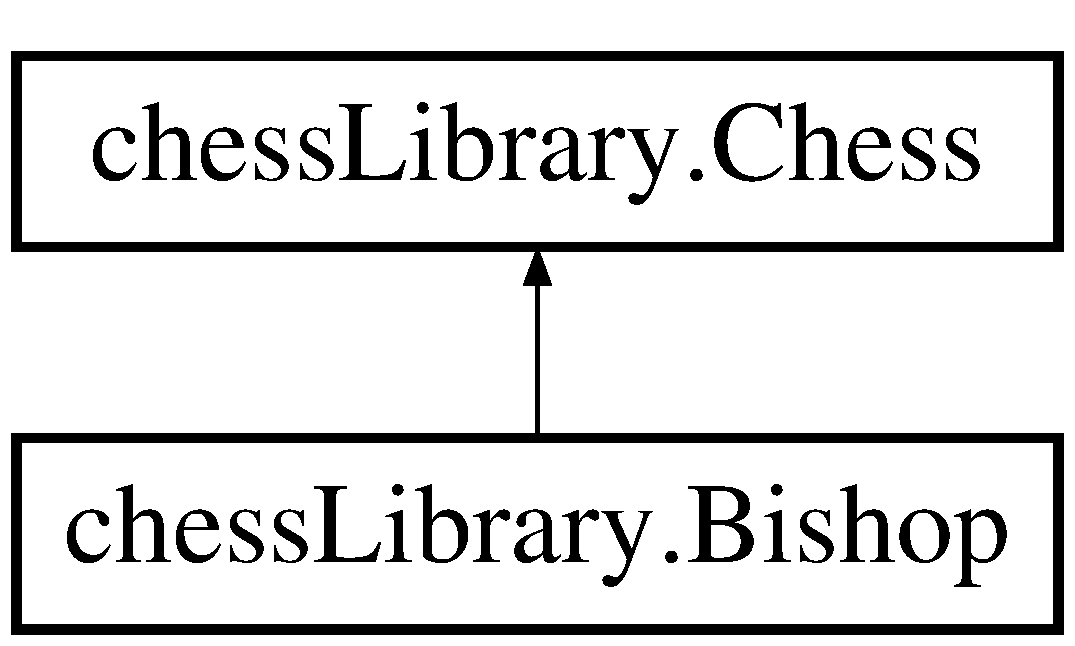
\includegraphics[height=2.000000cm]{classchess_library_1_1_bishop}
\end{center}
\end{figure}
\subsection*{Public Member Functions}
\begin{DoxyCompactItemize}
\item 
\mbox{\Hypertarget{classchess_library_1_1_bishop_a9eb76e95488ff2e8e7f17b3c1efc3a16}\label{classchess_library_1_1_bishop_a9eb76e95488ff2e8e7f17b3c1efc3a16}} 
{\bfseries Bishop} (int player, int row, int col)
\end{DoxyCompactItemize}
\subsection*{Additional Inherited Members}


The documentation for this class was generated from the following file\+:\begin{DoxyCompactItemize}
\item 
Bishop.\+java\end{DoxyCompactItemize}

\hypertarget{classchess_library_1_1_board}{}\section{chess\+Library.\+Board Class Reference}
\label{classchess_library_1_1_board}\index{chess\+Library.\+Board@{chess\+Library.\+Board}}
\subsection*{Public Member Functions}
\begin{DoxyCompactItemize}
\item 
\mbox{\Hypertarget{classchess_library_1_1_board_a55ccdb873f5bfacc82ad324e5e347a29}\label{classchess_library_1_1_board_a55ccdb873f5bfacc82ad324e5e347a29}} 
void {\bfseries move} (\hyperlink{classchess_library_1_1_chess}{Chess} piece, int row, int col)
\item 
\mbox{\Hypertarget{classchess_library_1_1_board_a519a32c78465562d7c0ebe874da270ae}\label{classchess_library_1_1_board_a519a32c78465562d7c0ebe874da270ae}} 
boolean {\bfseries detect\+Winner} (int player, int opponent)
\item 
\mbox{\Hypertarget{classchess_library_1_1_board_aef79046d600259559d6bfa0bc700114e}\label{classchess_library_1_1_board_aef79046d600259559d6bfa0bc700114e}} 
boolean {\bfseries try\+Move} (\hyperlink{classchess_library_1_1_chess}{Chess} piece, int new\+Row, int new\+Col)
\item 
\mbox{\Hypertarget{classchess_library_1_1_board_a7c009651ecd684c2f2cdd1a108316dae}\label{classchess_library_1_1_board_a7c009651ecd684c2f2cdd1a108316dae}} 
void {\bfseries set\+Position} (\hyperlink{classchess_library_1_1_chess}{Chess} piece, int new\+Row, int new\+Col, int curr\+Row, int curr\+Col)
\item 
\mbox{\Hypertarget{classchess_library_1_1_board_a791dfdec4490c444e1b22245e9957754}\label{classchess_library_1_1_board_a791dfdec4490c444e1b22245e9957754}} 
void {\bfseries capture\+Piece} (\hyperlink{classchess_library_1_1_chess}{Chess} piece)
\item 
\mbox{\Hypertarget{classchess_library_1_1_board_a3b5bdbec10a75b834d69576701b50f76}\label{classchess_library_1_1_board_a3b5bdbec10a75b834d69576701b50f76}} 
boolean {\bfseries check\+In\+Check} (int player)
\end{DoxyCompactItemize}
\subsection*{Static Public Member Functions}
\begin{DoxyCompactItemize}
\item 
\mbox{\Hypertarget{classchess_library_1_1_board_a8046eeea7ca2301ec44efd612863aa76}\label{classchess_library_1_1_board_a8046eeea7ca2301ec44efd612863aa76}} 
static void {\bfseries print\+Board} (\hyperlink{classchess_library_1_1_board}{Board} board)
\end{DoxyCompactItemize}
\subsection*{Public Attributes}
\begin{DoxyCompactItemize}
\item 
\mbox{\Hypertarget{classchess_library_1_1_board_aaa2ad24366b7716020708cd7e9fa54b0}\label{classchess_library_1_1_board_aaa2ad24366b7716020708cd7e9fa54b0}} 
boolean {\bfseries mute} = false
\item 
\mbox{\Hypertarget{classchess_library_1_1_board_aca7aa839370f2254fa8fb46f82996188}\label{classchess_library_1_1_board_aca7aa839370f2254fa8fb46f82996188}} 
\hyperlink{classchess_library_1_1_chess}{Chess} \mbox{[}$\,$\mbox{]}\mbox{[}$\,$\mbox{]} {\bfseries chess\+Position}
\item 
\mbox{\Hypertarget{classchess_library_1_1_board_ab65014a0c2f21c604819e2551bcd400b}\label{classchess_library_1_1_board_ab65014a0c2f21c604819e2551bcd400b}} 
\hyperlink{classchess_library_1_1_chess}{Chess} \mbox{[}$\,$\mbox{]}\mbox{[}$\,$\mbox{]} {\bfseries player\+Chess\+List}
\item 
\mbox{\Hypertarget{classchess_library_1_1_board_a3fd9afa635948753fc6609baab2b1239}\label{classchess_library_1_1_board_a3fd9afa635948753fc6609baab2b1239}} 
int {\bfseries turn} = 0
\item 
\mbox{\Hypertarget{classchess_library_1_1_board_a7cfa4b79e35c3f7baff0e2d584674ddc}\label{classchess_library_1_1_board_a7cfa4b79e35c3f7baff0e2d584674ddc}} 
int {\bfseries winning\+Player} =-\/1
\end{DoxyCompactItemize}
\subsection*{Static Public Attributes}
\begin{DoxyCompactItemize}
\item 
\mbox{\Hypertarget{classchess_library_1_1_board_a1bc8a3845eecddf03287e442369e0442}\label{classchess_library_1_1_board_a1bc8a3845eecddf03287e442369e0442}} 
static int {\bfseries board\+Size} = 8
\end{DoxyCompactItemize}


The documentation for this class was generated from the following file\+:\begin{DoxyCompactItemize}
\item 
Board.\+java\end{DoxyCompactItemize}

\hypertarget{classchess_library_1_1_chess}{}\section{chess\+Library.\+Chess Class Reference}
\label{classchess_library_1_1_chess}\index{chess\+Library.\+Chess@{chess\+Library.\+Chess}}
Inheritance diagram for chess\+Library.\+Chess\+:\begin{figure}[H]
\begin{center}
\leavevmode
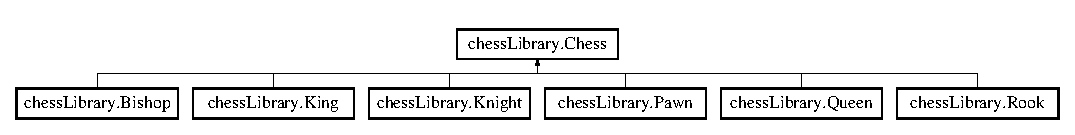
\includegraphics[height=1.372549cm]{classchess_library_1_1_chess}
\end{center}
\end{figure}
\subsection*{Public Member Functions}
\begin{DoxyCompactItemize}
\item 
\mbox{\Hypertarget{classchess_library_1_1_chess_a367823db5e0010dbc686f2589b5c3039}\label{classchess_library_1_1_chess_a367823db5e0010dbc686f2589b5c3039}} 
{\bfseries Chess} (int player, int row, int col)
\item 
\mbox{\Hypertarget{classchess_library_1_1_chess_a25fce16618d281a89acd51b824445396}\label{classchess_library_1_1_chess_a25fce16618d281a89acd51b824445396}} 
boolean {\bfseries check\+Rules\+For\+Test} (int new\+Row, int new\+Col)
\end{DoxyCompactItemize}
\subsection*{Public Attributes}
\begin{DoxyCompactItemize}
\item 
\mbox{\Hypertarget{classchess_library_1_1_chess_a2829345d8d3f38e26cecef4ab77919d6}\label{classchess_library_1_1_chess_a2829345d8d3f38e26cecef4ab77919d6}} 
int {\bfseries row}
\item 
\mbox{\Hypertarget{classchess_library_1_1_chess_a9c322dd6bd9d2cee433c82bdf876b3e8}\label{classchess_library_1_1_chess_a9c322dd6bd9d2cee433c82bdf876b3e8}} 
int {\bfseries col}
\item 
\mbox{\Hypertarget{classchess_library_1_1_chess_a2acefc2906f93c0da9aa3078a04e4c56}\label{classchess_library_1_1_chess_a2acefc2906f93c0da9aa3078a04e4c56}} 
boolean {\bfseries live}
\item 
\mbox{\Hypertarget{classchess_library_1_1_chess_a12759455cdf23360e8ecbd45ac81ca88}\label{classchess_library_1_1_chess_a12759455cdf23360e8ecbd45ac81ca88}} 
int {\bfseries player}
\item 
\mbox{\Hypertarget{classchess_library_1_1_chess_aad63de67e59fea708fe96532f9a615f2}\label{classchess_library_1_1_chess_aad63de67e59fea708fe96532f9a615f2}} 
char {\bfseries representive}
\end{DoxyCompactItemize}


The documentation for this class was generated from the following file\+:\begin{DoxyCompactItemize}
\item 
Chess.\+java\end{DoxyCompactItemize}

\hypertarget{classchess_library_1_1_king}{}\section{chess\+Library.\+King Class Reference}
\label{classchess_library_1_1_king}\index{chess\+Library.\+King@{chess\+Library.\+King}}
Inheritance diagram for chess\+Library.\+King\+:\begin{figure}[H]
\begin{center}
\leavevmode
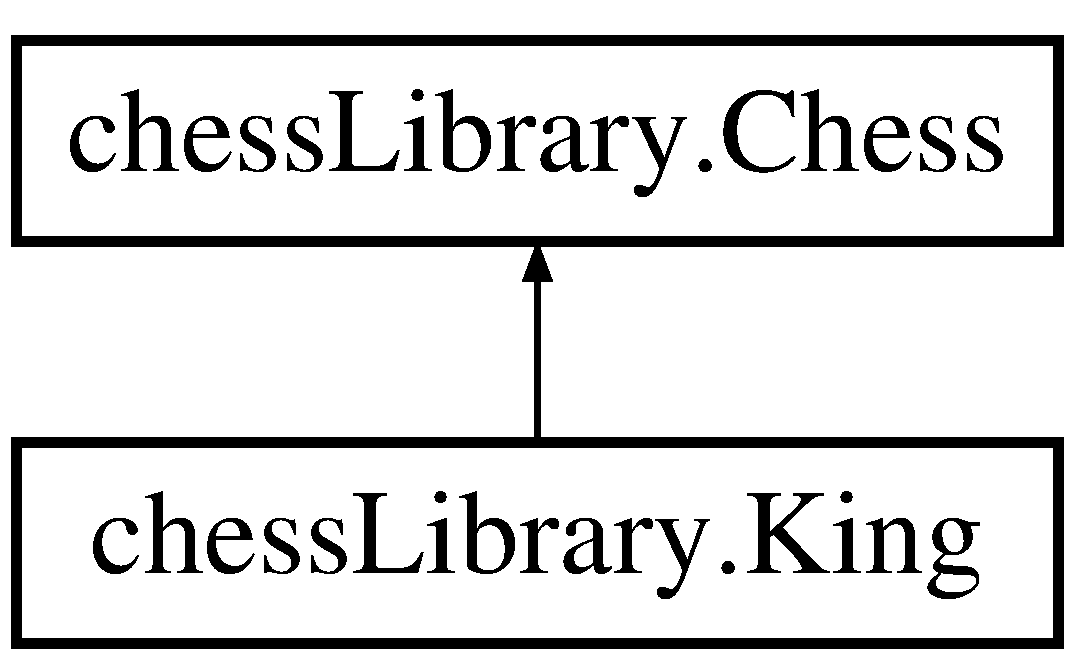
\includegraphics[height=2.000000cm]{classchess_library_1_1_king}
\end{center}
\end{figure}
\subsection*{Public Member Functions}
\begin{DoxyCompactItemize}
\item 
\mbox{\Hypertarget{classchess_library_1_1_king_aaf639a04c3d7b3a724229a56c2c5208d}\label{classchess_library_1_1_king_aaf639a04c3d7b3a724229a56c2c5208d}} 
{\bfseries King} (int player, int row, int col)
\end{DoxyCompactItemize}
\subsection*{Additional Inherited Members}


The documentation for this class was generated from the following file\+:\begin{DoxyCompactItemize}
\item 
King.\+java\end{DoxyCompactItemize}

\hypertarget{classchess_library_1_1_knight}{}\section{chess\+Library.\+Knight Class Reference}
\label{classchess_library_1_1_knight}\index{chess\+Library.\+Knight@{chess\+Library.\+Knight}}
Inheritance diagram for chess\+Library.\+Knight\+:\begin{figure}[H]
\begin{center}
\leavevmode
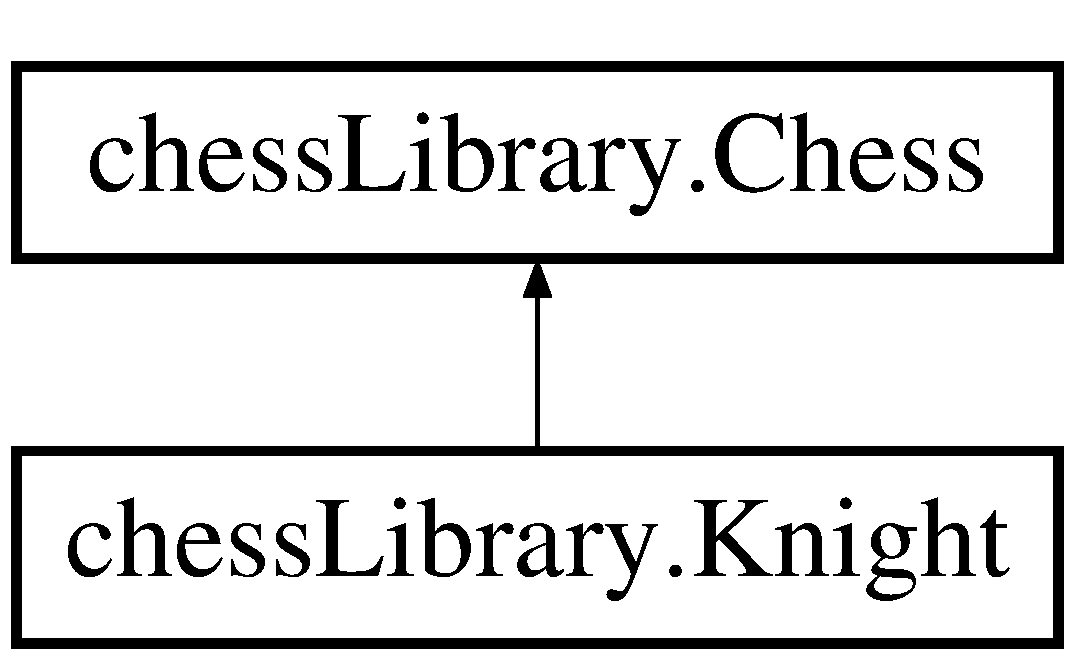
\includegraphics[height=2.000000cm]{classchess_library_1_1_knight}
\end{center}
\end{figure}
\subsection*{Public Member Functions}
\begin{DoxyCompactItemize}
\item 
\mbox{\Hypertarget{classchess_library_1_1_knight_a91cb9e4f33edf5ad275dccdd10199694}\label{classchess_library_1_1_knight_a91cb9e4f33edf5ad275dccdd10199694}} 
{\bfseries Knight} (int player, int row, int col)
\end{DoxyCompactItemize}
\subsection*{Additional Inherited Members}


The documentation for this class was generated from the following file\+:\begin{DoxyCompactItemize}
\item 
Knight.\+java\end{DoxyCompactItemize}

\hypertarget{classchess_library_1_1_pawn}{}\section{chess\+Library.\+Pawn Class Reference}
\label{classchess_library_1_1_pawn}\index{chess\+Library.\+Pawn@{chess\+Library.\+Pawn}}
Inheritance diagram for chess\+Library.\+Pawn\+:\begin{figure}[H]
\begin{center}
\leavevmode
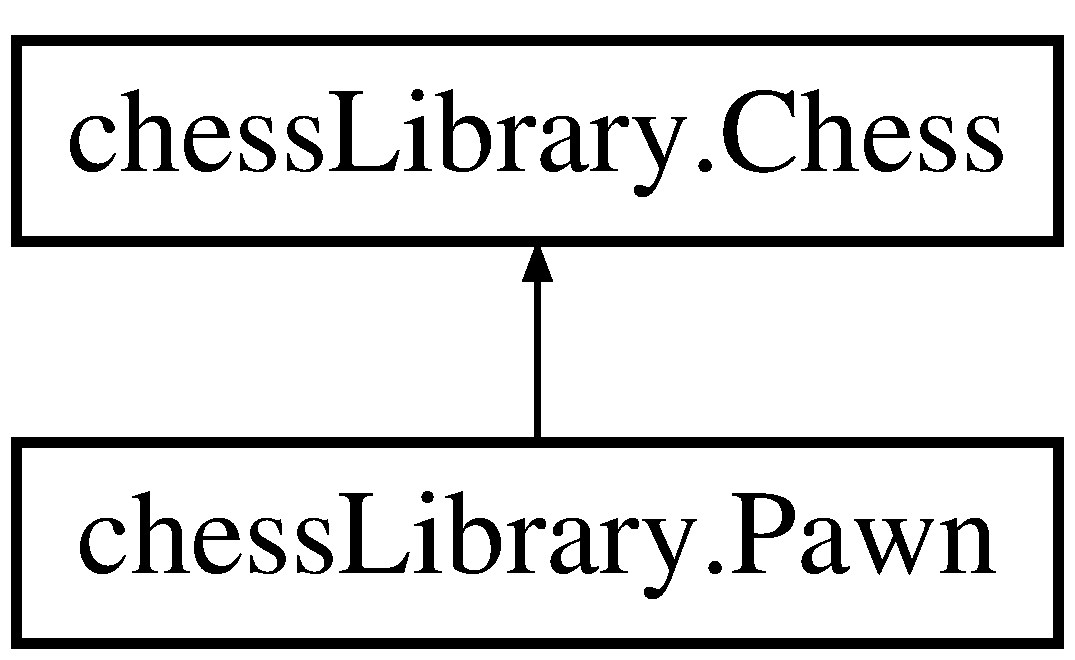
\includegraphics[height=2.000000cm]{classchess_library_1_1_pawn}
\end{center}
\end{figure}
\subsection*{Public Member Functions}
\begin{DoxyCompactItemize}
\item 
\mbox{\Hypertarget{classchess_library_1_1_pawn_a4109bd5acf3c39d99a3b77fcf2e92dfe}\label{classchess_library_1_1_pawn_a4109bd5acf3c39d99a3b77fcf2e92dfe}} 
{\bfseries Pawn} (int player, int row, int col)
\end{DoxyCompactItemize}
\subsection*{Additional Inherited Members}


The documentation for this class was generated from the following file\+:\begin{DoxyCompactItemize}
\item 
Pawn.\+java\end{DoxyCompactItemize}

\hypertarget{classchess_library_1_1_queen}{}\section{chess\+Library.\+Queen Class Reference}
\label{classchess_library_1_1_queen}\index{chess\+Library.\+Queen@{chess\+Library.\+Queen}}
Inheritance diagram for chess\+Library.\+Queen\+:\begin{figure}[H]
\begin{center}
\leavevmode
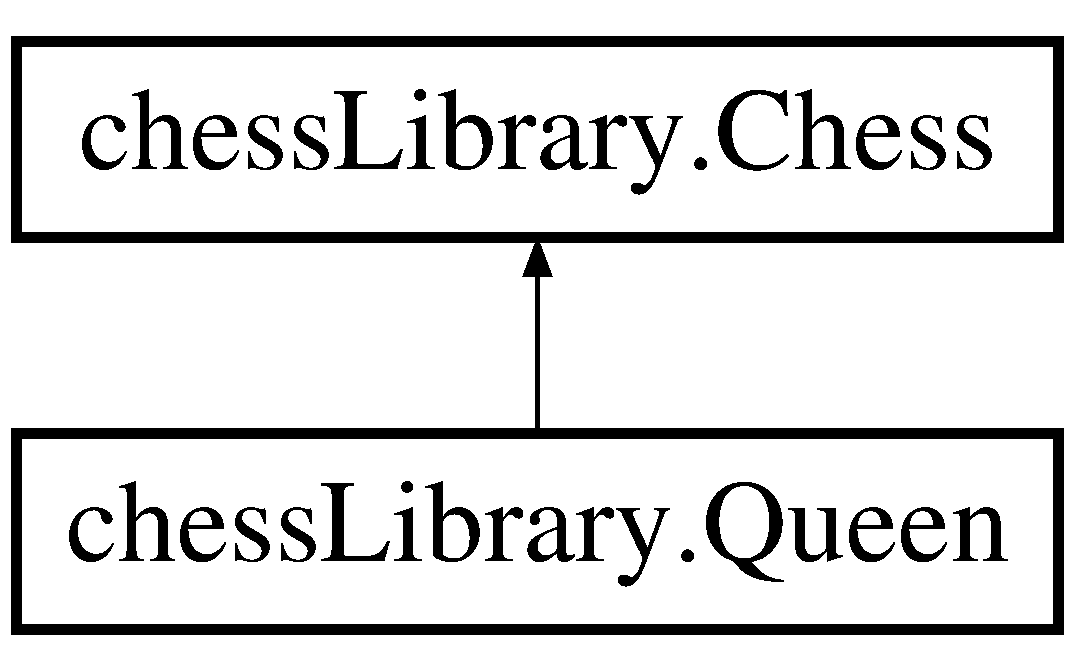
\includegraphics[height=2.000000cm]{classchess_library_1_1_queen}
\end{center}
\end{figure}
\subsection*{Public Member Functions}
\begin{DoxyCompactItemize}
\item 
\mbox{\Hypertarget{classchess_library_1_1_queen_a7e3627b5809de141b86895792a605ad1}\label{classchess_library_1_1_queen_a7e3627b5809de141b86895792a605ad1}} 
{\bfseries Queen} (int player, int row, int col)
\end{DoxyCompactItemize}
\subsection*{Additional Inherited Members}


The documentation for this class was generated from the following file\+:\begin{DoxyCompactItemize}
\item 
Queen.\+java\end{DoxyCompactItemize}

\hypertarget{classchess_library_1_1_rook}{}\section{chess\+Library.\+Rook Class Reference}
\label{classchess_library_1_1_rook}\index{chess\+Library.\+Rook@{chess\+Library.\+Rook}}
Inheritance diagram for chess\+Library.\+Rook\+:\begin{figure}[H]
\begin{center}
\leavevmode
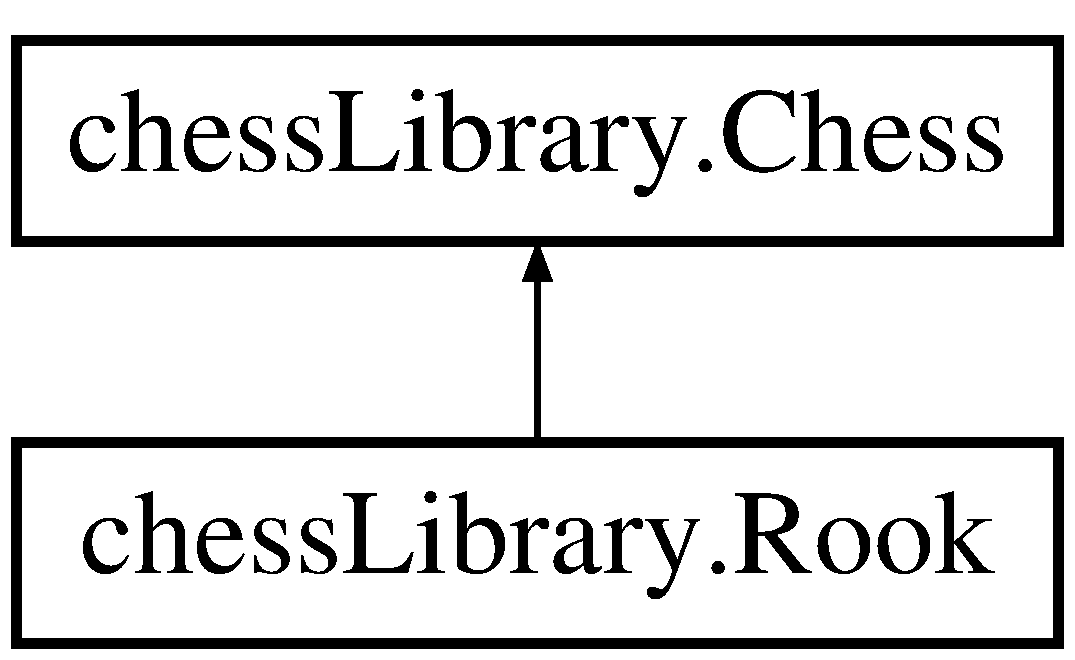
\includegraphics[height=2.000000cm]{classchess_library_1_1_rook}
\end{center}
\end{figure}
\subsection*{Public Member Functions}
\begin{DoxyCompactItemize}
\item 
\mbox{\Hypertarget{classchess_library_1_1_rook_a601989e504c3e3b63baa33da70fca8b5}\label{classchess_library_1_1_rook_a601989e504c3e3b63baa33da70fca8b5}} 
{\bfseries Rook} (int player, int row, int col)
\end{DoxyCompactItemize}
\subsection*{Additional Inherited Members}


The documentation for this class was generated from the following file\+:\begin{DoxyCompactItemize}
\item 
Rook.\+java\end{DoxyCompactItemize}

%--- End generated contents ---

% Index
\backmatter
\newpage
\phantomsection
\clearemptydoublepage
\addcontentsline{toc}{chapter}{Index}
\printindex

\end{document}
